% vim: spell spelllang=en:
%! TEX root = **/00-main.tex

% PCA analysis for numerical variables:

\section{PCA analysis for numerical variables}%
\label{sec:pca_analysis_for_numerical_variables}

% Scree plot. Specify how many principal components are selected
\subsection{Scree plot}%
\label{sub:scree_plot}


\begin{figure}[H]
    \centering
    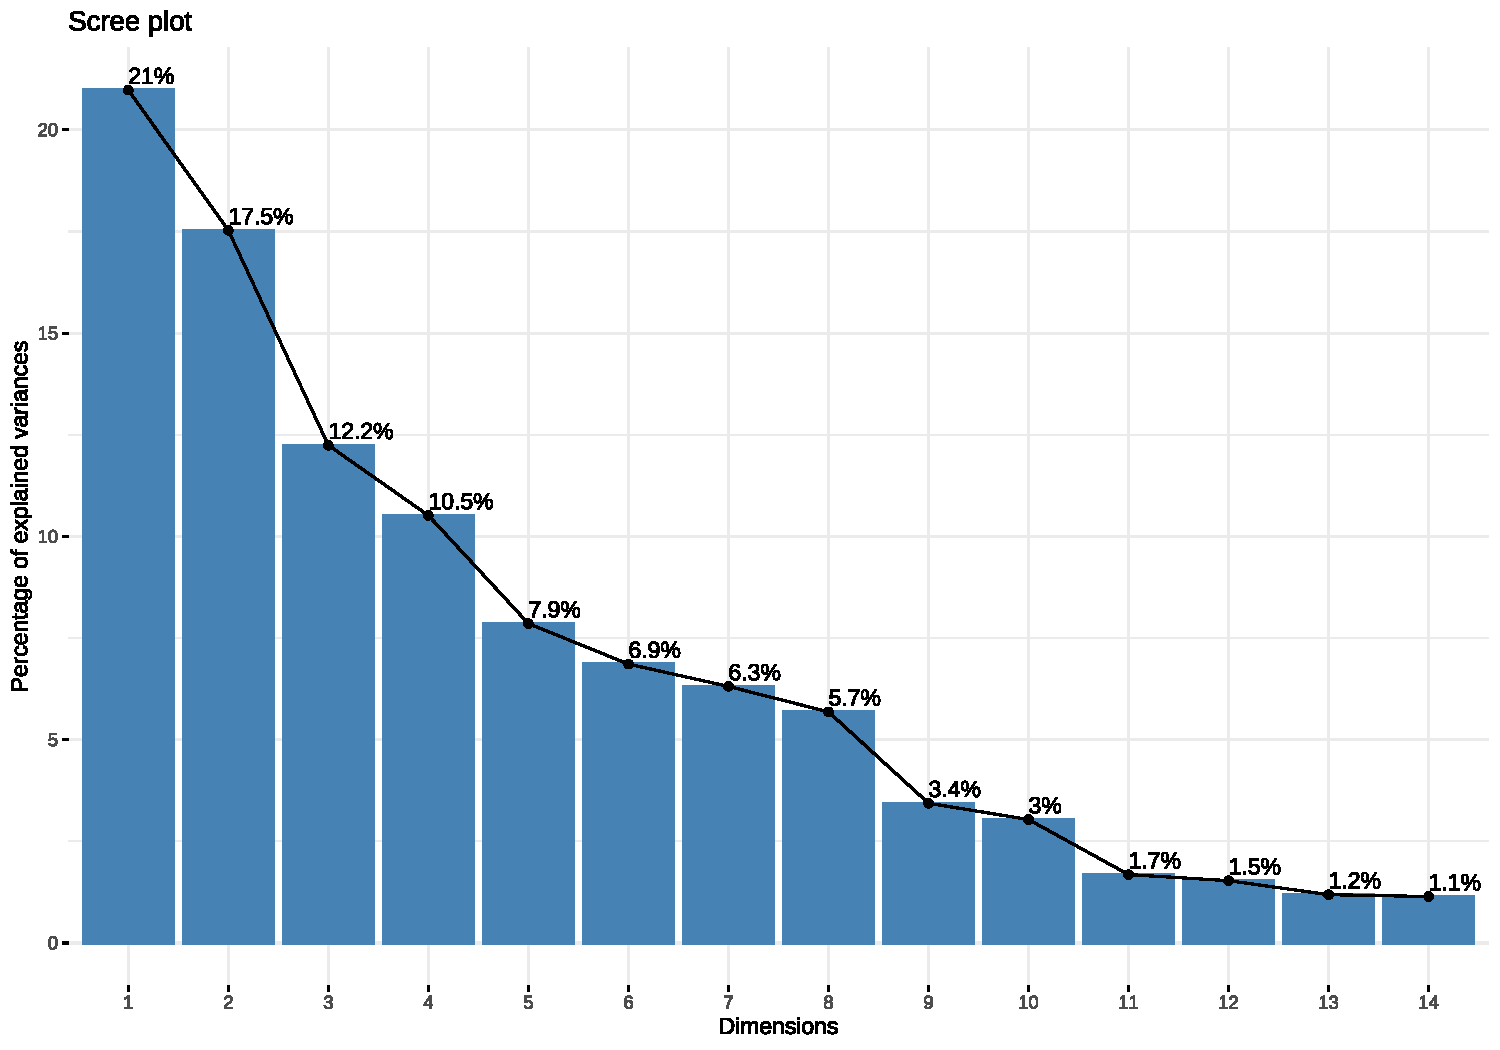
\includegraphics[width=0.7\linewidth]{pca_fact-screeplot} % PCA-inertia_cum
    \caption{PCA inertia}%
    \label{fig:pca_inertia}
\end{figure}

\begin{figure}[H]
    \centering
    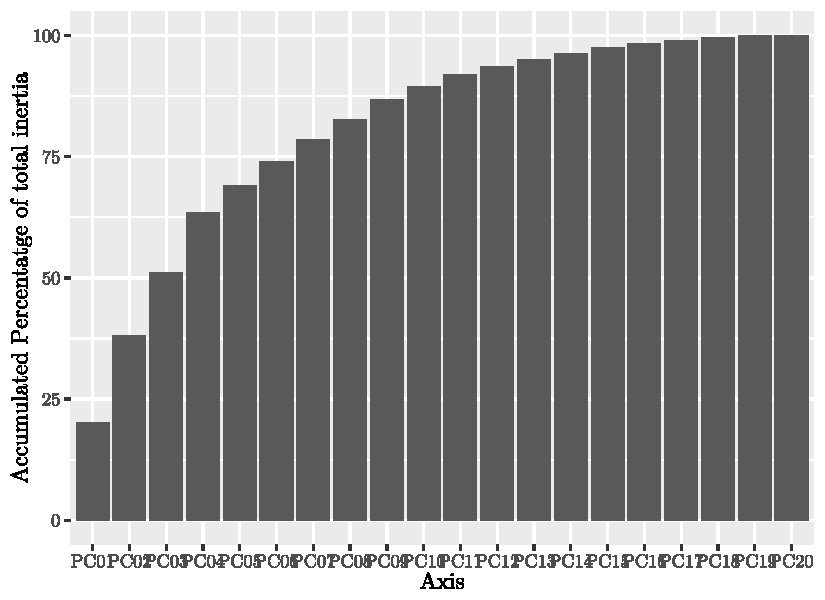
\includegraphics[width=0.7\linewidth]{PCA-inertia_cum}
    \caption{PCA accumulated inertia}%
    \label{fig:pca_inertia_cum}
\end{figure}

\vspace{-1em}
We used the inertia plots to decide the number of factorial axis to analyse. In
\cref{fig:pca_inertia} we can conclude the 4 first axis represent a much
larger amount of variance compared to the others. When looking at
\cref{fig:pca_inertia_cum} we can see that the first 4 axis already contain 63\%
of the variance. If we analyse further with the elbow method we can clearly see
that the slop starts to decrease at around the 4\ts{th} axis. Therefore we decided to
only further analyse the first 4 factorial axis.

% 20.24968405 17.88042469 13.04514781 12.39547495
% 20.24968  38.13011  51.17526  63.57073     %  69.09301  74.04671  78.51992  82.73880

\begin{table}[H]
    \centering
    \caption{Eigenvalues \& variance percentage of first 5 Dimensions}%
    \label{tab:eig}
    
\begin{tabular}[t]{lrrr}
\toprule
  & Eigenvalue & Var. \% & Cum. Var. \%\\
\midrule
comp 1 & 4.0499368 & 20.249684 & 20.24968\\
comp 2 & 3.5760849 & 17.880425 & 38.13011\\
comp 3 & 2.6090296 & 13.045148 & 51.17526\\
comp 4 & 2.4790950 & 12.395475 & 63.57073\\
comp 5 & 1.1044548 & 5.522274 & 69.09301\\
\addlinespace
comp 6 & 0.9907408 & 4.953704 & 74.04671\\
comp 7 & 0.8946421 & 4.473211 & 78.51992\\
comp 8 & 0.8437760 & 4.218880 & 82.73880\\
comp 9 & 0.8078400 & 4.039200 & 86.77800\\
comp 10 & 0.5511517 & 2.755759 & 89.53376\\
\bottomrule
\end{tabular}
\end{table}

\begin{table}[H]
    \centering
    \caption{Variable contribution to each axis}%
    \label{tab:}
    
\begin{tabular}[t]{lrrrr}
\toprule
  & Dim.1 & Dim.2 & Dim.3 & Dim.4\\
\midrule
host\_listings\_count & 1.1978839 & 0.2309859 & 1.2348477 & 1.9194330\\
accommodates & 1.7298781 & 4.9204820 & 15.4579382 & 8.8411427\\
bedrooms & 1.5035858 & 3.8248072 & 14.2067930 & 10.2701716\\
beds & 1.5539744 & 4.1550603 & 14.5044651 & 9.4446670\\
price & 0.3358423 & 0.5034663 & 1.7979068 & 2.5310976\\
\addlinespace
minimum\_nights\_avg\_ntm & 0.3285224 & 0.1053913 & 0.8458848 & 1.3083557\\
maximum\_nights\_avg\_ntm & 0.0326754 & 0.1551460 & 0.0180542 & 0.1915016\\
availability\_30 & 4.7100532 & 13.9585375 & 7.7416460 & 0.0782981\\
availability\_60 & 5.0921343 & 15.0338778 & 8.3809077 & 0.0804272\\
availability\_90 & 5.0164904 & 15.0703072 & 8.1727252 & 0.0732742\\
\addlinespace
availability\_365 & 3.9814077 & 9.6538067 & 2.9478169 & 0.0828489\\
number\_of\_reviews & 1.3671328 & 5.0656577 & 6.0696363 & 12.6128426\\
number\_of\_reviews\_ltm & 1.4742472 & 5.9390691 & 6.6049015 & 15.9807855\\
number\_of\_reviews\_l30d & 0.3293267 & 1.6735082 & 1.7305596 & 5.7081947\\
review\_scores\_rating & 16.2922433 & 2.7642390 & 1.0363407 & 3.3113763\\
\addlinespace
review\_scores\_accuracy & 15.2310328 & 2.7062625 & 0.7857840 & 2.4644208\\
review\_scores\_cleanliness & 12.6689566 & 3.1473241 & 0.5491346 & 2.7145276\\
review\_scores\_location & 9.5058782 & 2.5671720 & 0.4498178 & 1.7099762\\
review\_scores\_value & 15.7847912 & 2.5825171 & 1.1601061 & 2.4687109\\
reviews\_per\_month & 1.8639432 & 5.9423821 & 6.3047340 & 18.2079477\\
\bottomrule
\end{tabular}
\end{table}

% Factorial map visualisation:
\subsection{Factorial map visualisation}%
\label{sub:factorial_map_visualisation}

% #2 -> caption #3 -> file, #1 -> page
\newcommand{\factorialmap}[2]{
    \begin{landscape}
    \begin{figure}[H]
        \centering
        \includegraphics[width=0.87\linewidth]{pca_fact-plane_#1_#2-bi}
        \caption{PCA plane #1 vs #2}%
        \label{fig:plane_#1-#2}
    \end{figure}
    \end{landscape}
}

\newcommand{\factvar}[2]{
    \begin{figure}[H]
        \centering
        \includegraphics[width=0.67\textwidth]{pca_fact-plane_#1_#2-var}
        \caption{PCA plane #1 vs #2 (numerical)}%
        \label{fig:plane_#1-#2-var}
    \end{figure}
}

\newcommand{\factorialmapCV}[2]{
    \contrib{#1}{#2}
    \factvar{#1}{#2}
}

\newcommand{\contrib}[2]{
    \begin{figure}[H]
        \centering
        \includegraphics[width=0.85\linewidth]{pca_fact-plane_#1_#2-contrib}
        \caption{PCA variable contributions of plane #1 vs #2}%
        \label{fig:contrib_plane_#1-#2}
    \end{figure}
}

\newcommand{\categorica}[4]{
    \begin{figure}[H]
        \centering
        \includegraphics[width=0.85\linewidth]{pca_fact-#3-plane_#1_#2}
        \caption{PCA variable contributions of #4 in plane #1 vs #2}%
        \label{fig:cat-#3-plane-#1-#2}
    \end{figure}
}

%TODO

\factorialmap{1}{2}
In \cref{fig:plane_1-2} we are showing the factorial maps that represent the most variance among all our factorial axis. When looking at the numerical variables represented we can see that all there are some variables that tend to be grouped. For example
there's a group about all review scores, another with beds, bedroom and accommodates and another with availabilities. When 
analysing \cref{fig:contrib_plane_1-2} we can see that accommodates, beds and the review scores are top contributors to
this plane. When analysing the contribution to each plane it's clear that review scores are affecting mostly axis 2, whereas accommodates and beds mostly affect axis 1.

\begin{comment}
In \cref{fig:plane_1-2} we are showing the factorial maps that represent the most variance among all our factorial axis. When looking at the numerical variables represented we can see that all the variables
related to reviews tend to have similar arrows, this makes sense 
because in the bivariate analysis we concluded that they were correlated.
Looking at \cref{fig:contrib_plane_1-2} we can see that the variables
with higher contribution are the ones about review scores and availability. As all review score variables have a small angle to the first factorial axis we can begin to speculate that this axis is 
mostly affected by these variables. Other variables like availability
and accommodates seem to contribute mostly to the second factorial axis, however these angles aren't as tight so they probably affect the first axis as well. 
\end{comment}
\factorialmapCV{1}{2}


\factorialmap{1}{3}
In \cref{fig:plane_1-3} we can see that it seems to hold true that the accommodates and beds affects axis 1 the most. Price 
seems to have a similar arrow as those variables. This might be
because there is some correlation between those variables. 
(The more beds a house has, probably the more expensive it is).
The arrows of variables about number of reviews have a very small angle with factorial axis 3. Minimum\_nights\_avg\_ntm seem to
be affecting axis 3 as well but inversely.

\factorialmapCV{1}{3}

\factorialmap{1}{4}

In \cref{fig:plane_1-4} we can see that again it is true
the accommodates and beds variables affects axis 1 the most. We can begin to speculate that these might be factorial axis 1
latent variables. Looking at \cref{fig:contrib_plane_1-4} we 
can see that availabities first appear as top contributors and seem to be related with the forth factorial axis.

\begin{comment}
The plane in \cref{fig:plane_1-4} seems to be mostly affected by review scores and the number of reviews.
In this specific plane number of reviews and accommodates seem to have a similar contribution but with
inverse relation. We can maybe relate the availability with the first plane, but as the global correlation
to this plane of this variable isn't has high we can't derive to much from this.
\end{comment}

\factorialmapCV{1}{4}


\factorialmap{2}{3}
%TODO
In \cref{fig:contrib_plane_2-3} the most contributing variables are the availabilities, accommodates and bedrooms.
These particular plot doesn't help us much in regards to finding associations with the axis because the
angles the variables form are too wide.
\factorialmapCV{2}{3}


\factorialmap{2}{4}

What we can extract when analysing \cref{fig:plane_2-4} is that the availability variables have 
a relatively high contribution and form a very small angle with the forth factorial axis. The same happens with review scores and the second axis.

\factorialmapCV{2}{4}


\factorialmap{3}{4}
We can't extract much more from \cref{fig:plane_3-4}. Everything
aforementioned seems to hold true in this specific plane.

\factorialmapCV{3}{4}

\begin{landscape}

\categorica{1}{2}{room_type}{room type}
\categorica{1}{3}{room_type}{room type}
\categorica{1}{4}{room_type}{room type}

\end{landscape}

\subsection{Conclusion}%
What we can conclude after analysing how the variables are distributed along each factorial axis is 
that our variables generally distribute in 4 groups: the ones about availability, 
the ones about review scores, the ones regarding number of reviews and finally beds and accommodation. That might happen
because there is some correlation between them.

After studying each factorial axis in depth we can concluded that the latent variables associated to 
the first factorial map are the ones that talk about review scores. We reached these conclusion after
seeing that in all PCA plots with with the first factorial axis, these variables were top contributors
and their angles to the first axis were really small. The relation seems to be direct as in all plots 
they appear in the positive first axis. Although this relation appears in all plots where factorial
axis 1 appears we think \cref{fig:plane_1-3} depicts this relation the best. 

We conclude that the PCA visualization was an overall success because we were able to detect some grouped
variables and relate some of them to our factorial axis. In fact, we ended up associating the first axis
with the review score variables. This is a major success because the first factorial axis is the one
that represents more variance and therefore associating a meaning to it could help us better explain
out variables.


% (Be sure you use a single landscape pager for each single map in order to
% guarantee visibility of materials to the readers)

% For each factorial map provide:

% - Individuals projections

% - Common projection of numerical variables and modalities of qualitative
% - variables (take care to use correct color codes as explained along the course)

% - Interpretation of relationships among variables observed. When possible,
% - interpret the latent variable associated with the principal axis

% - Conclusions

% Note: All factorial maps must be placed in a single landscape page that makes
% it visible
